\documentclass[8pt]{beamer}

% Der Plan
% Folie 1: Introduction: Henry
% Folie 2: Dataset: Christopher
% Folie 3: Network Architecture: Christopher
% Folie 4: Hyperparameter: Christopher
% Folie 5: Overtraining: Christopher
% Folie 6: Results: Henry
% Folie 7: Alternative Methods: Henry
% Folie 8: Conclusion: Henry
% Appendix: ???

% unverzichtbare Mathe-Befehle
\usepackage{amsmath}
% viele Mathe-Symbole
\usepackage{amssymb}
% Erweiterungen für amsmath
\usepackage{mathtools}

% Fonteinstellungen
\usepackage{fontspec}
% Latin Modern Fonts werden automatisch geladen

% deutsche Spracheinstellungen
% \usepackage[ngerman]{babel}
\usepackage[english]{babel}
%BUG in Biblatex wird hiermit gefixt
\providetoggle{blx@lang@captions@english}

\usepackage[
  math-style=ISO,    % ┐
  bold-style=ISO,    % │
  sans-style=italic, % │ ISO-Standard folgen
  nabla=upright,     % │
  partial=upright,   % ┘
  warnings-off={           % ┐
    mathtools-colon,       % │ unnötige Warnungen ausschalten
    mathtools-overbracket, % │
  },                       % ┘
]{unicode-math}

% traditionelle Fonts für Mathematik
\setmathfont{Latin Modern Math}
\setmathfont{XITS Math}[range={scr, bfscr}]
\setmathfont{XITS Math}[range={cal, bfcal}, StylisticSet=1]

% Zahlen und Einheiten
\usepackage[
  % locale=DE,                   % deutsche Einstellungen
  locale=US,
  separate-uncertainty=true,   % immer Fehler mit \pm
  per-mode=symbol-or-fraction, % / in inline math, fraction in display math
]{siunitx}

% richtige Anführungszeichen
\usepackage[autostyle]{csquotes}

% schöne Brüche im Text
\usepackage{xfrac}

% Grafiken können eingebunden werden
\usepackage{graphicx}

% Grafiken können in LaTex gemalt werden
\usepackage{tikz, pgfplots}

% Ermöglicht relative Positionierung von tikz-Nodes
\usetikzlibrary{positioning}

% Für Feynman-Graphen mit Tikz
\usepackage{feynmp-auto}

% Für komplexere Captions
\usepackage{caption}

% Literaturverzeichnis
\usepackage[
  backend=biber,
  style=authoryear,
  autocite=inline,
]{biblatex}
% Quellendatenbank
\addbibresource{presentation.bib}

\usetheme[numbering=fraction]{metropolis}

% Für die Titelseite
%\title{The Influence of Music Genres on Performance Metrics: A Comparative Analysis of Spotify and YouTube}
\title{The Genre Factor}
\subtitle{Project Presentation - ML Seminar 2023}
\author{Henry Krämerkämper\\%
  \and%
  Christopher Breitfeld}
\institute{Technische Universität Dortmund}
\date{13.07.2023}
\logo{
\includegraphics[height=0.5cm]{figures/tu_logo_sw_klein.pdf}}

\begin{document}

\begin{frame}
  \titlepage
\end{frame}

\begin{frame}
\frametitle{Introduction to the Problem}
  \begin{columns}
  \column{0.5\textwidth}
    \begin{itemize}
      \item Genre classification of songs based on audio features
      \item Dataset: Thousands of songs with diverse genres
      \item Challenge: Developing an accurate classification model
    \end{itemize}
  \column{0.5\textwidth}
    \begin{figure}
      \centering
      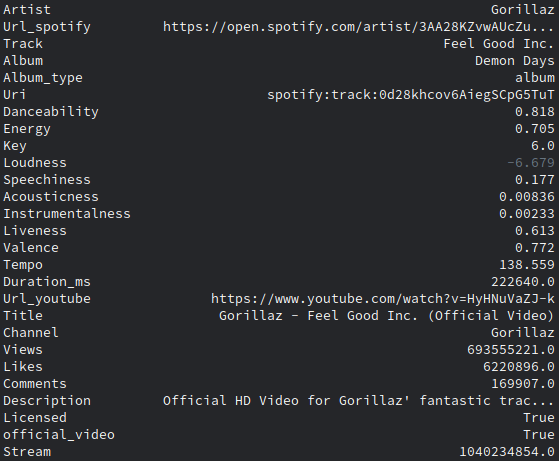
\includegraphics[scale=0.3]{figures/Beispielsong.png}
      \caption{Example of a song and its attributes.}
    \end{figure}
  \end{columns}
\end{frame}

\begin{frame}{Description of the Data Set}
  \begin{alertblock}{Dataset from \href{https://www.kaggle.com/datasets/salvatorerastelli/spotify-and-youtube}{Kaggle}: Spotify and YouTube}
	\begin{itemize}
      \item Contains statistics of songs on Spotify and YouTube
      \item including streams on Spotify and number of views on YouTube
      \item 20.7k entries by 2k artists
      \item Does \alert{NOT} include the genre
      \item Licensed under CC0: Public Domain
    \end{itemize}
  \end{alertblock}
  \begin{alertblock}{Wikidata Query for the Top-Genre of the Artist}
	\begin{itemize}
     \item Query artist's Wikidata page for genre names
     \item Choose a list of broader genres, so that the genres are not too specific
     \item Match artist to one of the genres on the list, based on the query
     \item Usage possible under CC-by-SA-3.0
    \end{itemize}
  \end{alertblock}
  \begin{alertblock}{Target of the resulting Dataset}
	\begin{itemize}
     \item Target: genre
    \end{itemize}
  \end{alertblock}
\end{frame}


\begin{frame}
\frametitle{Network Architecture}

\begin{itemize}
\item Neural network model for genre classification
\item Layers, activation functions, and number of parameters
\item Training process and optimization algorithm
\end{itemize}

\end{frame}

\begin{frame}
\frametitle{Hyperparameter Optimization}

\begin{itemize}
\item Importance of hyperparameter tuning
\item Methods used (e.g., grid search, random search)
\item Results of optimization and best hyperparameters
\end{itemize}

\end{frame}

\begin{frame}
\frametitle{Overtraining Checks}

\begin{itemize}
\item Preventing overfitting in the model
\item Regularization techniques used (e.g., dropout, weight decay)
\item Validation and test set performance
\end{itemize}

\end{frame}

\begin{frame}
\frametitle{Results of our Neural Network}
\begin{figure}<1>
  \centering
  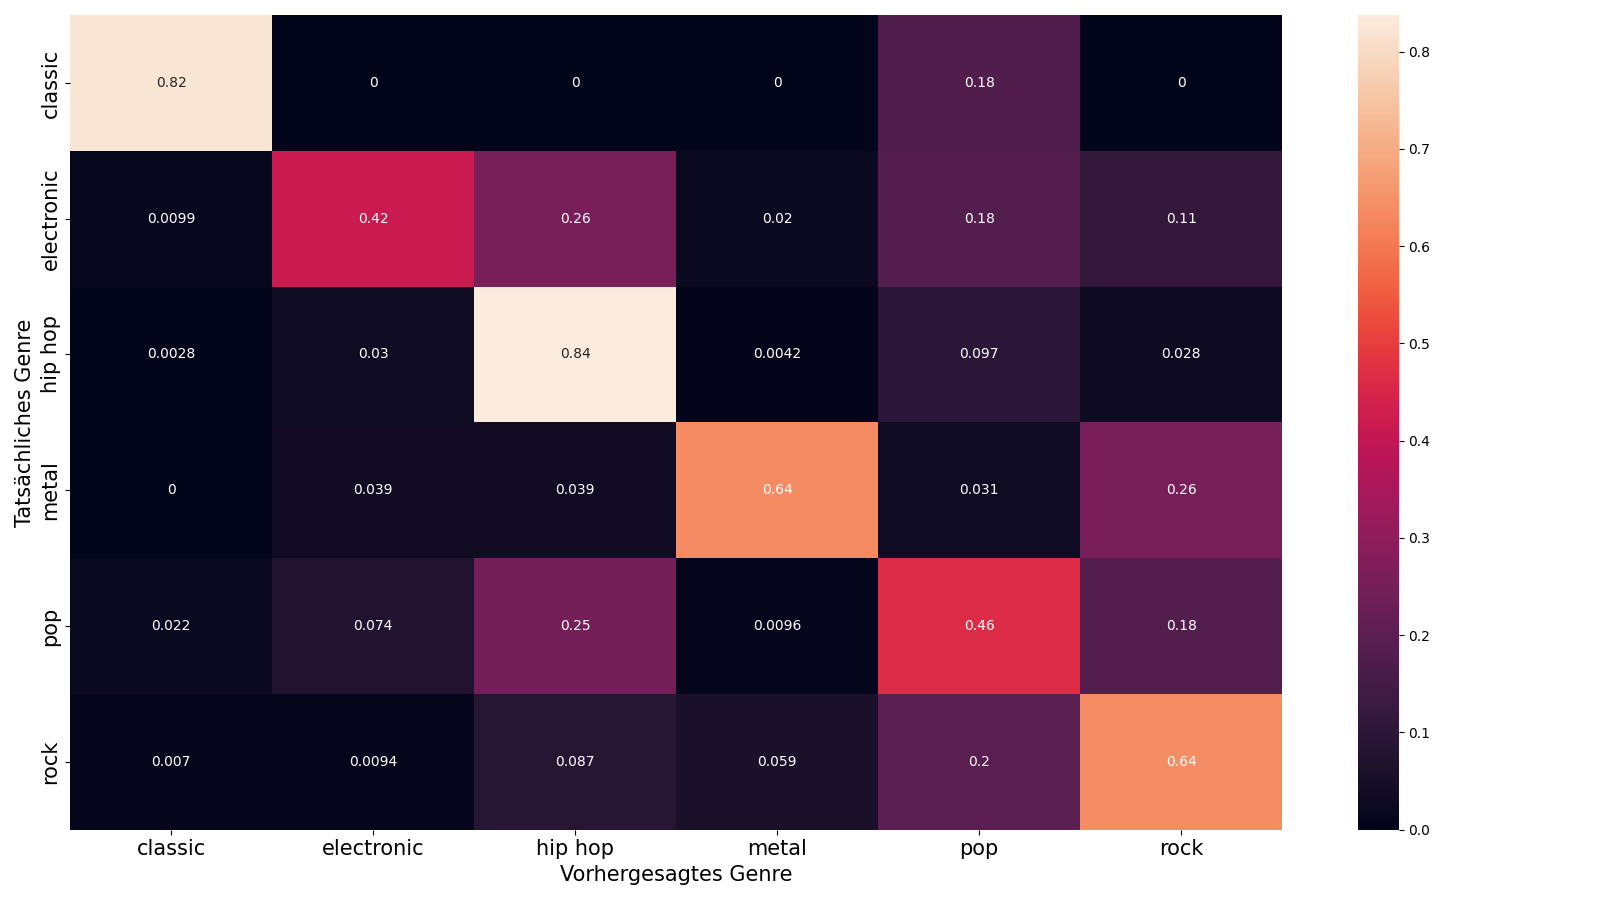
\includegraphics[scale=0.32]{figures/confusion_matrix_NN.png}
\end{figure}
\begin{alertblock}{Accuracy and AUC-PR}<2->
	\begin{itemize}
   \item Results in an accuracy of $\SI{65.87}{\percent}$ on test data
   \item As well as an AUC-PR score of $\num{0.738}$
  \end{itemize}
\end{alertblock}
\end{frame}

\begin{frame}
\frametitle{Alternative Methods}
  \begin{alertblock}{K-nearest-neighbors}
    \begin{itemize}
     \item We use $k=12$ as it achieves the highest performance
     \item Results in an accuracy of $\SI{60.62}{\percent}$
    \end{itemize}
  \end{alertblock}
  \begin{alertblock}{Support vector machines}
    \begin{itemize}
    \item{model that classifies data by finding the hyperplane that maximally separates different categories in a multidimensional space}
    \item We use an One-vs-One approach to be able to do Multiclass-Classification:
    \begin{itemize}
      \item A separate model is trained for each pair of classes, and a given data point is classified by majority voting among the classifiers
      \end{itemize}
    \item The used kernel function is the radial basis function (RBF)
    \item Results in an accuracy of $\SI{63.88}{\percent}$
    \end{itemize}
  \end{alertblock}
\end{frame}

\begin{frame}
\frametitle{Conclusions}
  \begin{itemize}
          \item NN achieves an accuracy of $\SI{65.87}{\percent}$ on test data.
          \item Diminishing returns for more complex models, we are constrained by the dataset
  \end{itemize}
  \begin{figure}
    \centering
    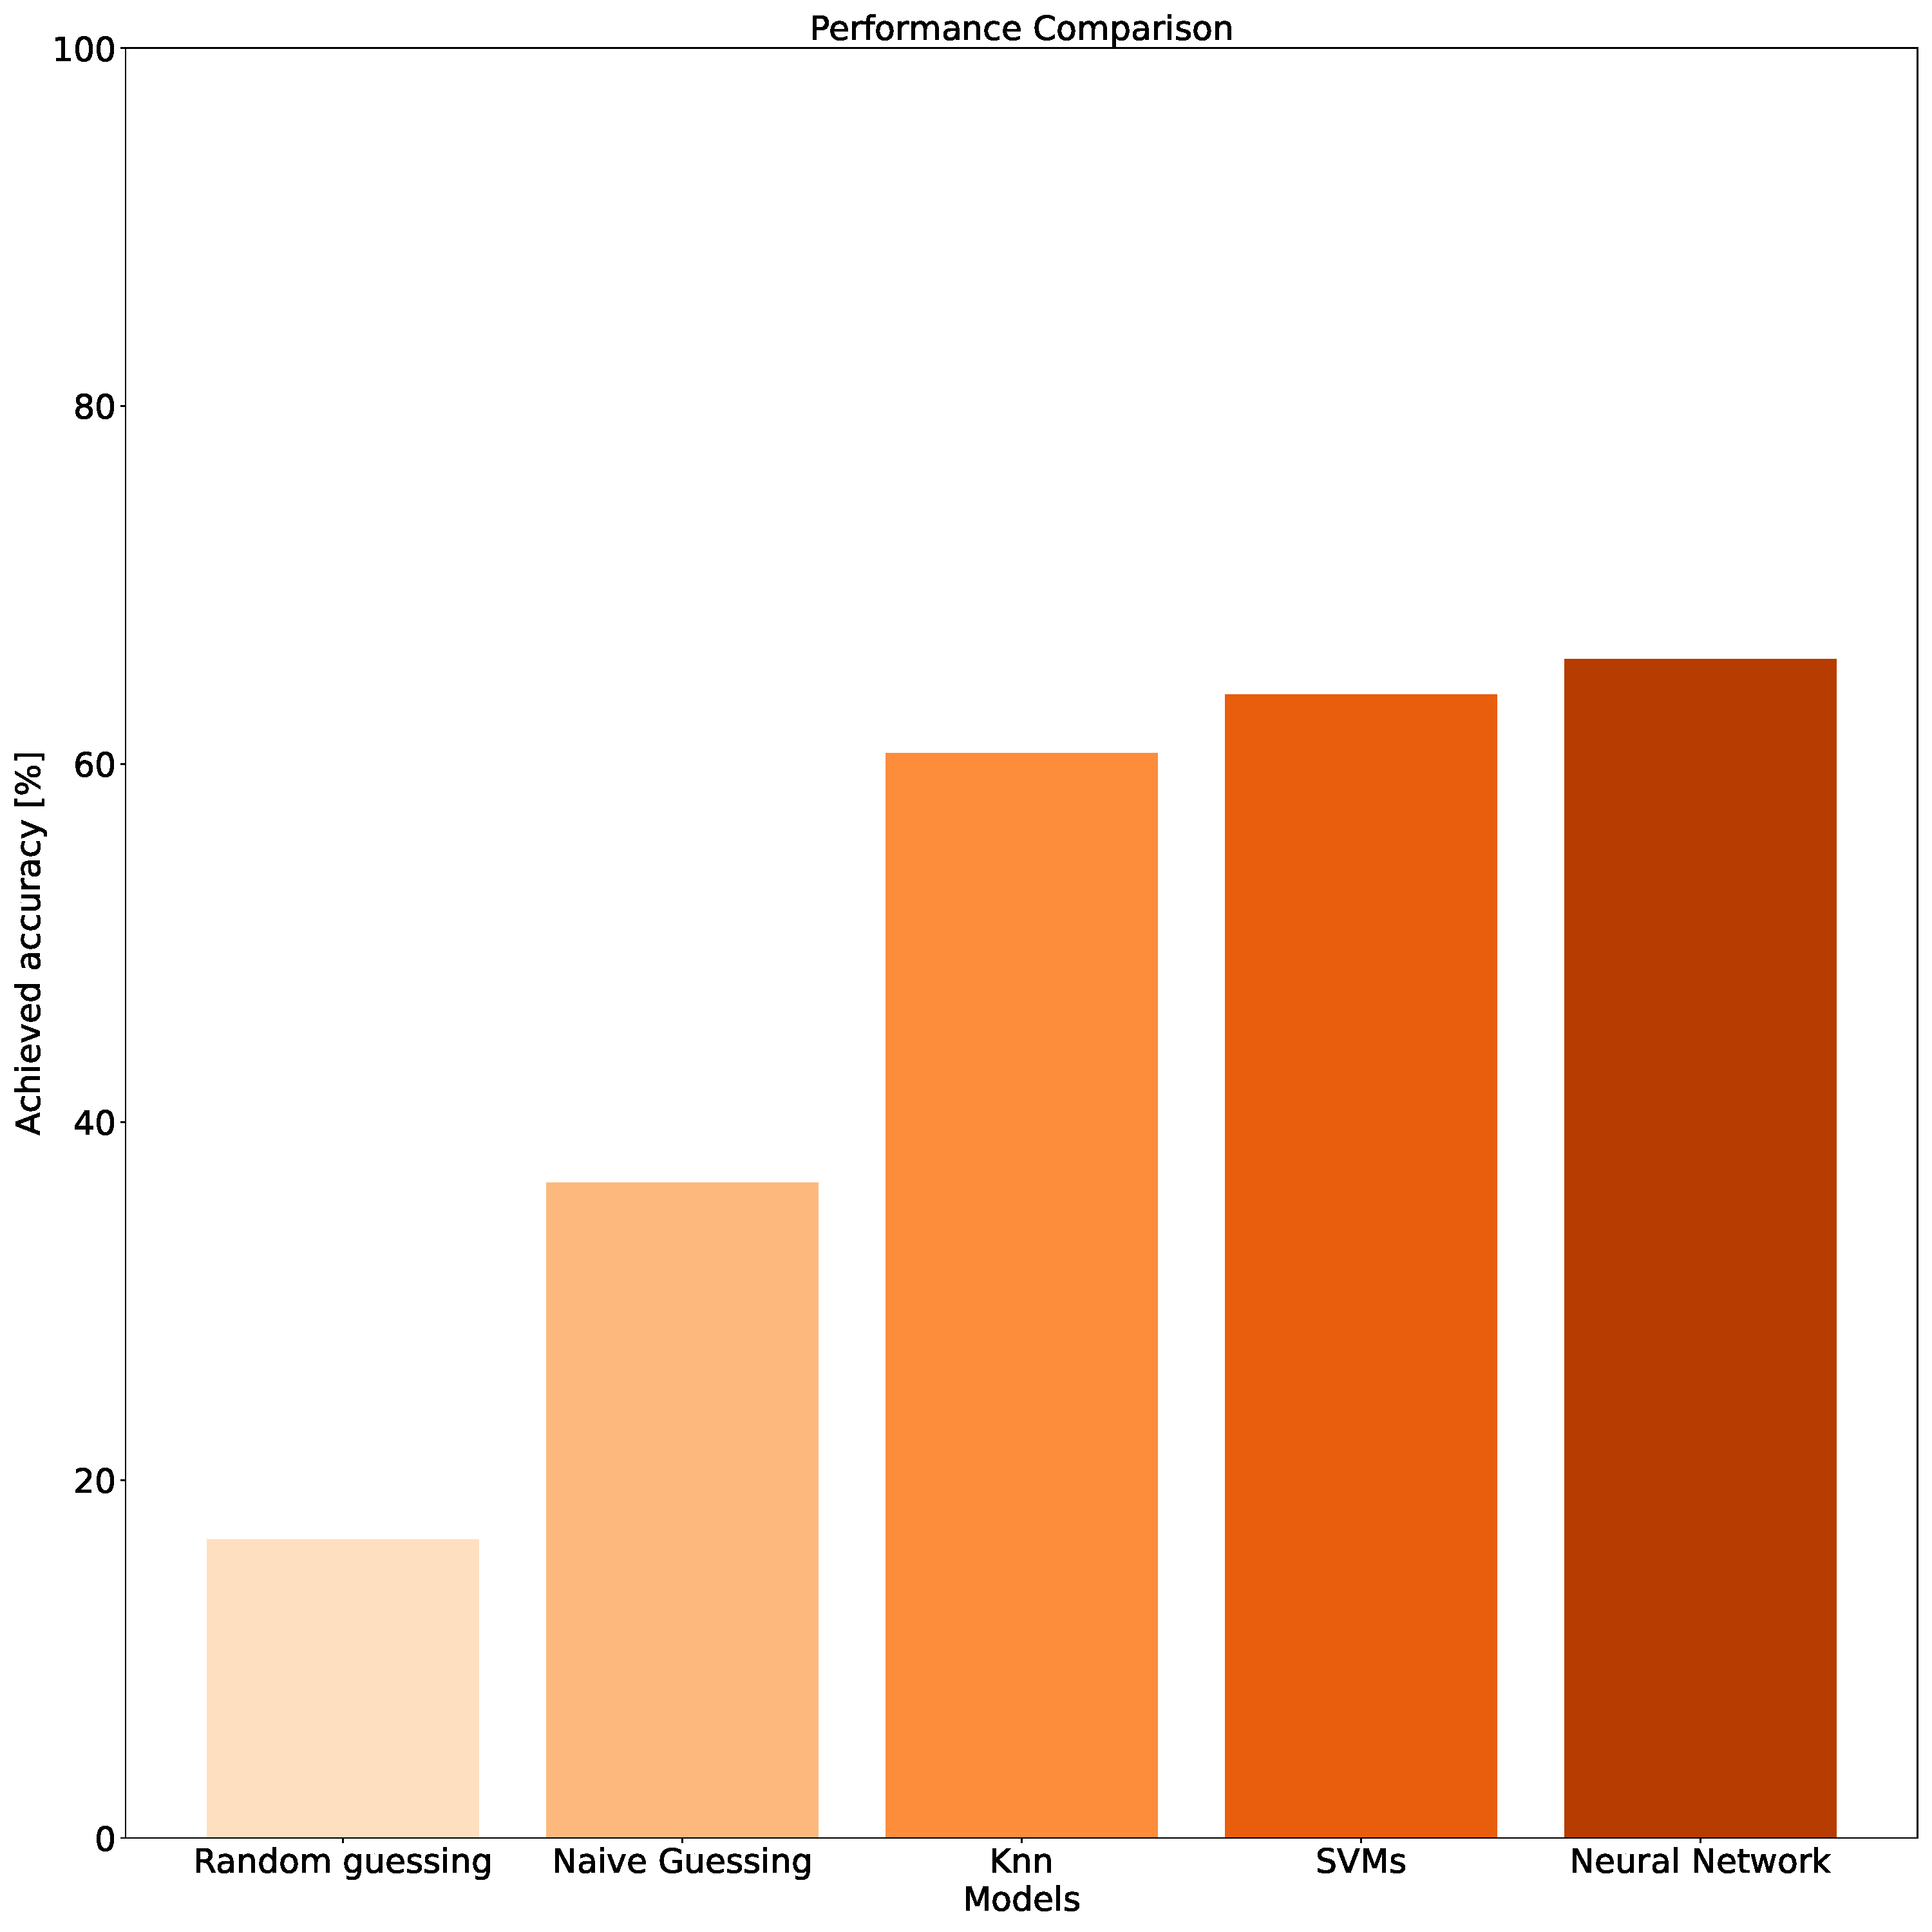
\includegraphics[scale=0.15]{figures/performance-comparison.pdf}
    % \caption{Comparison of the accuracy of different approaches.}
  \end{figure}
\end{frame}

% Alle Quellen, die bisher nicht zitiert wurden
%\nocite{Theories_of_grbs}

\printbibliography

\appendix
\begin{frame}{Appendix: The features of our dataset}
  \begin{alertblock}{Features}
    \begin{columns}[t]
      \begin{column}{0.5\textwidth}
        \begin{itemize}
          \item Track
          \item Artist
          \item Url\_Spotify 
          \item Album 
          \item Album\_type 
          \item Uri 
          \item Danceability
          \item Energy 
          \item Key 
          \item Loudness 
          \item Speechiness 
          \item Acousticness 
          \item Instrumentalness
          \item Liveness 
          \item Tempo 
        \end{itemize}
      \end{column}
      \begin{column}{0.5\textwidth}
        \begin{itemize}
          \item Duration\_ms 
          \item Stream 
          \item Url\_youtube 
          \item Title 
          \item Channel
          \item Views 
          \item Likes 
          \item Comments 
          \item Description 
          \item Licensed
          \item official\_video
        \end{itemize}
      \end{column}
    \end{columns}
  \end{alertblock}
\end{frame}

% \begin{frame}{Appendix: Das Synchrotron Burnoff Limit}

% \end{frame}

% \begin{frame}{Appendix: Detektion eines Gammablitzes: Methoden}

% \end{frame}

% \begin{frame}{Appendix: Detektion eines Gammablitzes: Schwierigkeiten}

% \end{frame}

\end{document}
